\documentclass[../main.tex]{subfiles}

\begin{document}

\section*{Appendex A: Visualization Exemplars}

Appendex A includes a typology of data visualizations which may be supported within DAVE workbooks.
These visualizations can either be one to one or one to many in regards to the algorithms defined within this document.
Future iterations of this document will increasingly include these typologies within the domain-question template exemplars.

\section*{Line Charts}

\begin{figure*}[h]
  \centering
  {\caption{Line Chart}
    \label{fig1}}
  {\begin{tikzpicture}
      \begin{axis}
        \addplot+[sharp plot] coordinates
        {(0,0) (1,2) (2,3)};
      \end{axis}
    \end{tikzpicture}}
\end{figure*}

\begin{figure*}[h]
  \centering
  {\caption {Line Chart with Error}
    \label{fig2}}
  {\begin{tikzpicture}
      \begin{axis}
        \addplot+[error bars/.cd,x dir=both,x explicit]
        coordinates {
          (0,0)   +- (0.1,0)
          (0.5,1) +- (0.4,0.2)
          (1,2)
          (2,5)   +- (1,0.1)
        };
      \end{axis}
    \end{tikzpicture}}
\end{figure*}

\begin{figure*}[h]
  \centering
  {\caption{Spline Chart}
    \label{fig3}}
  {\begin{tikzpicture}
      \begin{axis}[nodes near coords={(\coordindex)}]
        \addplot[mark=*, patch,mesh, patch type=cubic spline]
        coordinates {
          % left, right, left middle, right middle
          (-1,-1)
          (1,1)
          (-1/3,{(-1/3)^3})
          (1/3,{(1/3)^3})};
      \end{axis}
    \end{tikzpicture}}
\end{figure*}

\begin{figure*}[h]
  \centering
  {\caption{Quiver Chart}
    \label{Fig4}}
  {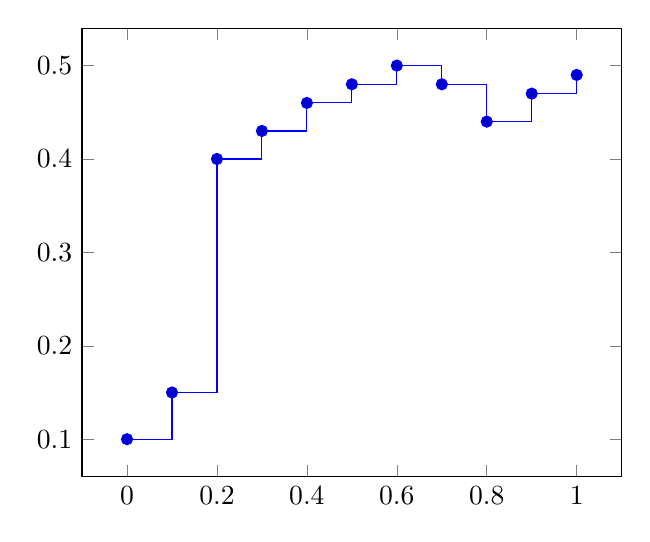
\begin{tikzpicture}
      \begin{axis}
        \addplot+[const plot]
        coordinates
        {(0,0.1)    (0.1,0.15)  (0.2,0.4)   (0.3,0.43)
          (0.4,0.46) (0.5,0.48)  (0.6,0.50)  (0.7,0.48)
          (0.8,0.44) (0.9,0.47)  (1,0.49)};
      \end{axis}
    \end{tikzpicture}}
\end{figure*}
\FloatBarrier

\section*{Grouping Charts}

\begin{figure*}[h]
  \centering
  {\caption{Grouped Line Charts}
    \label{Fig5}}
  {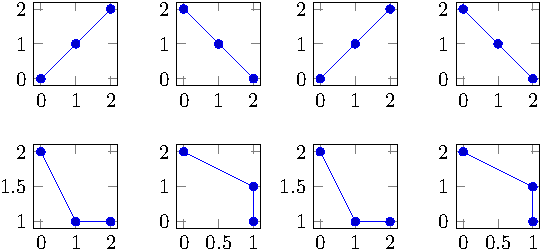
\includegraphics[page=1]{multiple_line.pdf}}
\end{figure*}

\begin{figure*}[h]
  \centering
  {\caption{Histogram}
    \label{fig6}}
  {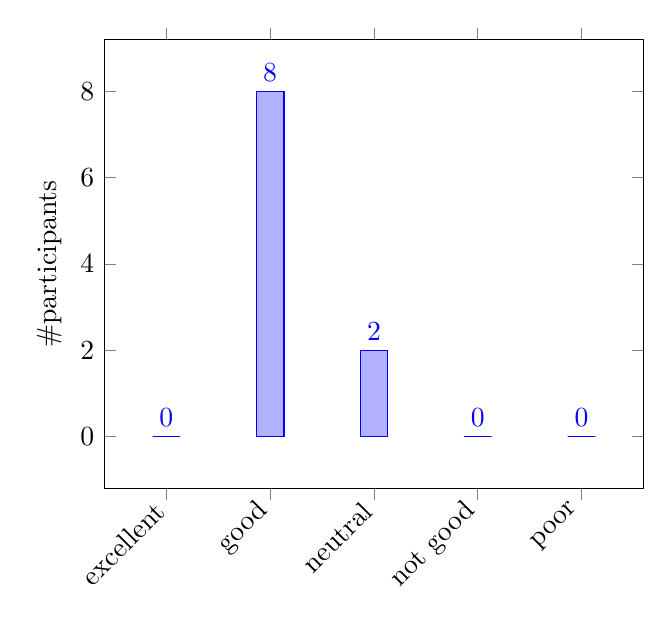
\begin{tikzpicture}
      \begin{axis}[
        ybar,
        enlargelimits=0.15,
        legend style={at={(0.5,-0.2)},
          anchor=north,legend columns=-1},
        ylabel={\#participants},
        symbolic x coords={excellent,good,neutral, not good,poor},
        xtick=data,
        nodes near coords,
        nodes near coords align={vertical},
        x tick label style={rotate=45,anchor=east},
        ]
        \addplot coordinates {(excellent,0) (good,8)
          (neutral,2) (not good,0) (poor,0)};
      \end{axis}
    \end{tikzpicture}}
\end{figure*}

\begin{figure*}[h]
  \centering
  {\caption{Bar Chart}
    \label{fig7}}
  {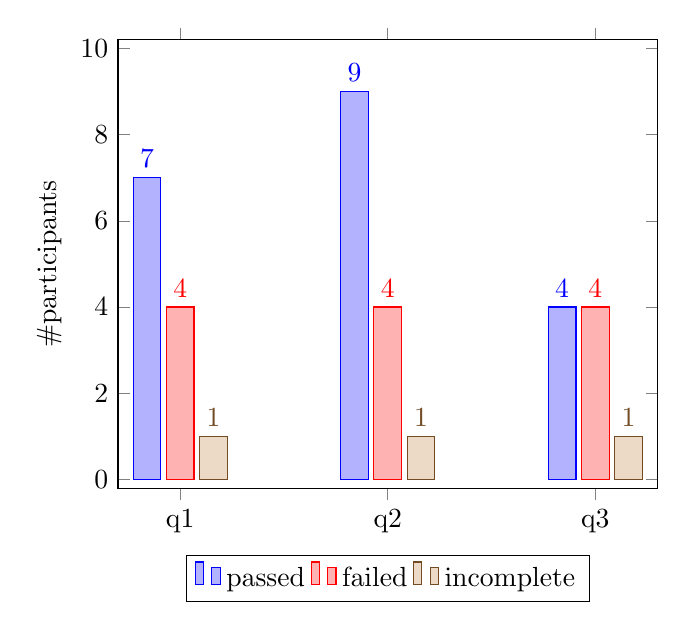
\begin{tikzpicture}
      \begin{axis}[
        ybar,
        enlargelimits=0.15,
        legend style={at={(0.5,-0.15)},
          anchor=north,legend columns=-1},
        ylabel={\#participants},
        symbolic x coords={q1,q2,q3},
        xtick=data,
        nodes near coords,
        nodes near coords align={vertical},
        ]
        \addplot coordinates {(q1,7) (q2,9) (q3,4)};
        \addplot coordinates {(q1,4) (q2,4) (q3,4)};
        \addplot coordinates {(q1,1) (q2,1) (q3,1)};
        \legend{passed,failed,incomplete}
      \end{axis}
    \end{tikzpicture}}
\end{figure*}

\begin{figure*}[h]
  \centering
  {\caption{Bar Chart Grouped by Time Range}
    \label{fig8}}
  {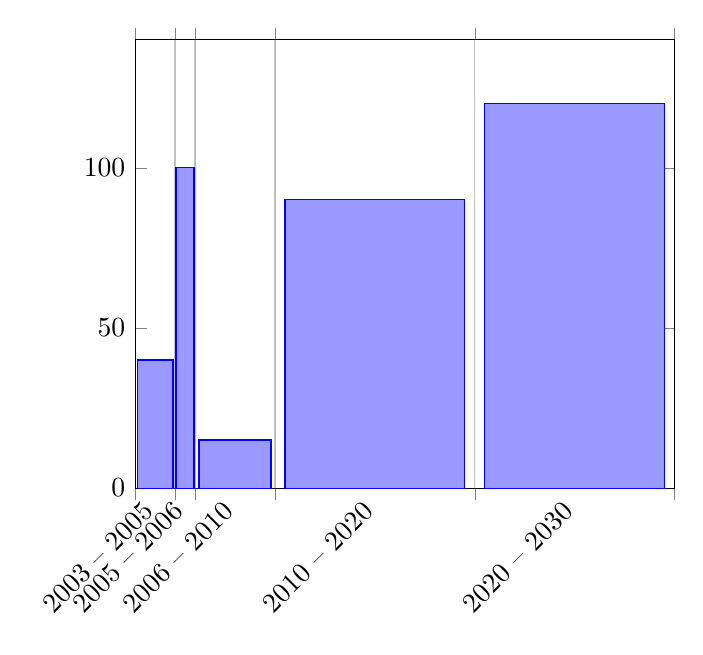
\begin{tikzpicture}
      \begin{axis}[
        ybar interval=0.9,
        x tick label as interval,
        xmin=2003,xmax=2030,
        ymin=0,ymax=140,
        xticklabel={
          $\pgfmathprintnumber{\tick}$
          -- $\pgfmathprintnumber{\nexttick}$},
        xtick=data,
        x tick label style={
          rotate=45,anchor=east,
          /pgf/number format/1000 sep=}]
        \addplot[draw=blue,fill=blue!40!white]
        coordinates
        {(2003,40) (2005,100) (2006,15)
          (2010,90) (2020,120) (2030,3)};
      \end{axis}
    \end{tikzpicture}}
\end{figure*}

\begin{figure*}[h]
  \centering
  {\caption{Scatter Plot}
    \label{fig9}}
  {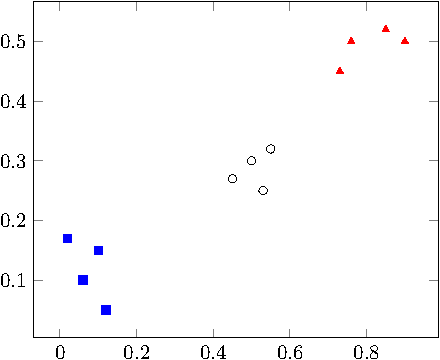
\includegraphics[page=1]{scatter_plot.pdf}}
\end{figure*}

\begin{figure*}[h]
  \centering
  {\caption{Polar Chart}
    \label{fig10}}
    {\begin{tikzpicture}
        \begin{polaraxis}
          \addplot+[polar comb]
          coordinates {(300,1) (20,0.3) (40,0.5)
            (120,1) (200,0.4)};
        \end{polaraxis}
      \end{tikzpicture}}
\end{figure*}

\section*{Specialized Charts}

\begin{figure*}[h]
  \centering
  {\caption{Gantt Chart}\label{fig11}}
    {\begin{tikzpicture}
        \begin{axis}[xtick=\empty, ytick=\empty]
          \addplot+
          [jump mark left]
          coordinates
          {(0,12) (1,9) (2,8) (3,5) (4,3) (5,1)};
        \end{axis}
      \end{tikzpicture}}
\end{figure*}

\begin{figure*}[h]
  \centering
  {\caption{Heat Map}
    \label{fig12}}
    {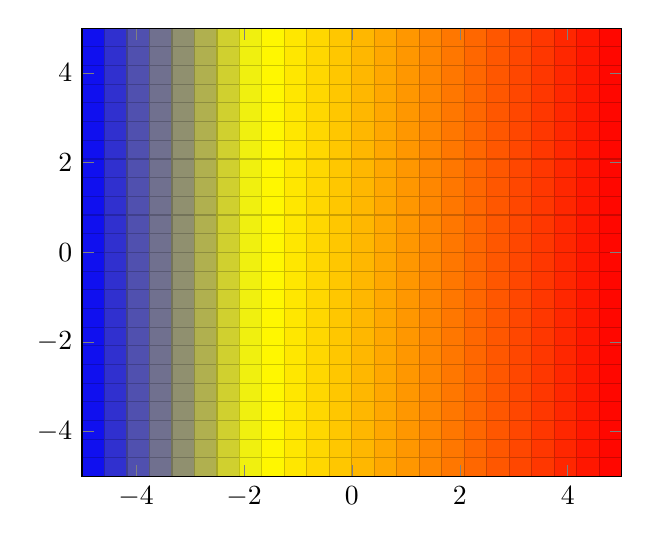
\begin{tikzpicture}
	\begin{axis}[view={0}{90}]
          \addplot3[surf] {x};
	\end{axis}
      \end{tikzpicture}}
\end{figure*}

\begin{figure*}[h]
  \centering
  {\caption{3D Plot}
    \label{fig13}}
  {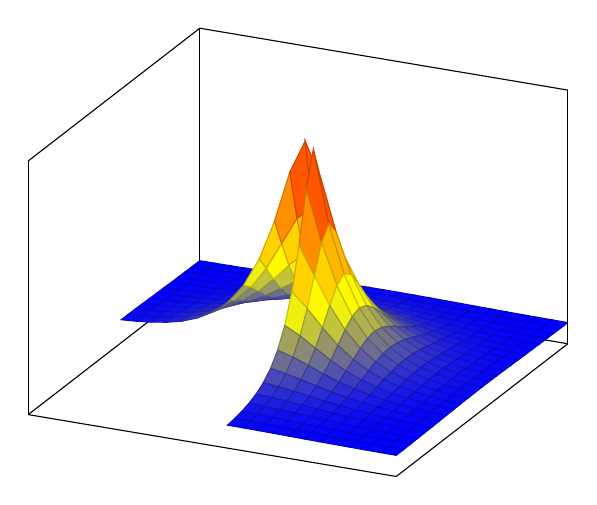
\begin{tikzpicture}
        \begin{axis}[
          xtick=\empty, ytick=\empty, ztick=\empty,
          unbounded coords=jump,
          % A technical filter to cut out
          % the x<0 and y<0 edge.
          filter point/.code={%
            \pgfmathparse
            {\pgfkeysvalueof{/data point/x}<0}%
            \ifpgfmathfloatcomparison
            \pgfmathparse
            {\pgfkeysvalueof{/data point/y}<0}%
            \ifpgfmathfloatcomparison
            \pgfkeyssetvalue{/data point/x}{nan}%
            \fi
            \fi
          },
          ]
          \addplot3[surf] {exp(-sqrt(x^2 + y^2))};
        \end{axis}
      \end{tikzpicture}}
  \end{figure*}

  \begin{figure*}[h]
    \centering
    {\caption{Gradient Plot}
      \label{fig13}}
    {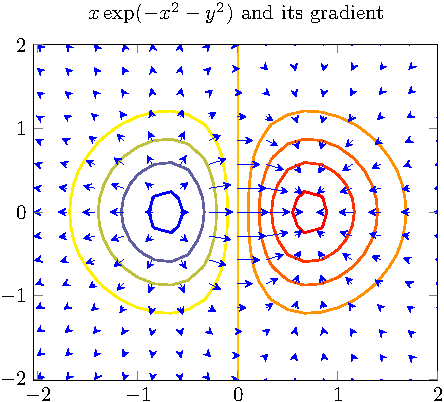
\includegraphics[page=1]{gradient.pdf}}
    \end{figure*}

\end{document}
